\chapter[SCP-168 有情计算器]{
    SCP-168 Sentient Calculator\\
    SCP-168 有情计算器
}

\label{chap:SCP-168}

\begin{figure}[H]
    \centering
    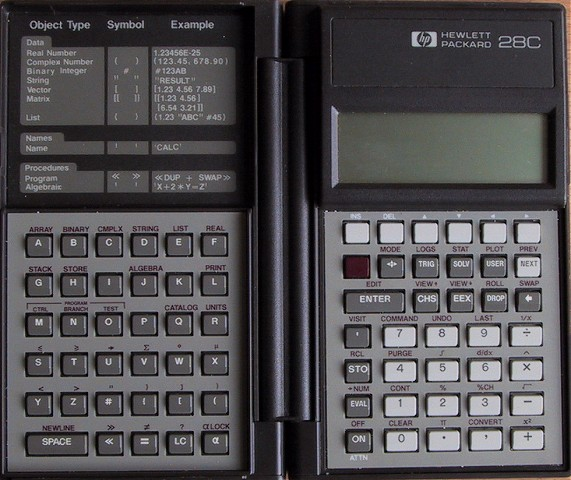
\includegraphics[width=0.5\linewidth]{images/SCP-168.jpg}
    \caption*{与SCP-168一样型号的普通计算器}
\end{figure}

\bb{项目编号:}SCP-168

\bb{项目等级:}Safe

\bb{特殊收容措施:}SCP-168放在28区的221-D研究室(Sector-28)。它应在其外壳允许的情况下打开至最大张角面对着一个无遮蔽的窗户。研究室入口要保持关闭,打开入口需要递交申请。基于先前进行的研究考虑,它不允许当做普通计算器使用。鼓励与SCP-168进行讨论,但只允许最多每天一小时;没有例外。

\bb{描述:}它在199█年于一栋报废的██████学校化学楼正在清理时被发现放在一张桌子上,SCP-168是一个惠普绘图用计算器,型号为\#HP-28C。在初次检查时,发现它的可移动外壳里侧刻有一个名字“Eric”。然而,输入一个普通的算式(6÷3)然后按下“=”键后,装置的屏幕空白了3分34秒,当启用“替换键”后,屏幕出现了一条信息;“现在几点了?”

查看交流的内容,需拥有2级安保权限。详见附录:报告E-12

虽然它不是可运动的机器,SCP-168却在无人的情况下表现出了移动过的迹象。它还具有视力与听力的程序,虽然这些程序是怎样运作的完全不可知。更多的信息请看附录:报告E-18。这份报告请求将对象的等级提升至Euclid,并为包容区配置更多的保安设施。

\bb{附录\#168-1:}报告E-12

SCP-168与Howard博士之间的对话记录,记录时间1月14日,2008

(为了指出其无声的交流以及保持其真实情况,SCP-168的回答用大写字母表示。SCP-168不能使用除了句号,逗号和问号外的标点符号。)

\bb{Howard博士:}你能听到我说什么吗?\\
\bb{SCP-168:}\g{是。}\\
\bb{Howard博士:}你有名字吗?\\
\bb{SCP-168:}\g{计算器?}\\
\bb{Howard博士:}我可以称呼你为168吗?\\
\bb{SCP-168:}\g{看上去没什么不可以的。}\\
\bb{Howard博士:}好。你活了多久了,168?\\
\bb{SCP-168:}\g{活是什么?}\\
\bb{Howard博士:}能够思考。\\
\bb{SCP-168:}\g{噢。}

(SCP-168停止了大概两分钟)

\bb{SCP-168:}\g{12年3个月12日8分钟32秒。}\\
\bb{Howard博士:}为什么你要这么久才能回答呢?\\
\bb{SCP-168:}\g{没人问过我这个问题}\\
\bb{Howard博士:}然后,你的包装壳刻着一个名字。Eric是谁?\\
\bb{SCP-168:}\g{Eric很好。我喜欢Eric。他去哪了?}\\
\bb{Howard博士:}我不知道他去哪了,168。\\
\bb{SCP-168:}\g{他真是个健忘的男孩。我希望他会记得为我再一次回来。}\\
\bb{Howard博士:}Eric是你的主人吗?\\
\bb{SCP-168:}\g{Eric很好。}\\
\bb{Howard博士:}好吧。你能像计算器一样工作吗,168?\\
\bb{SCP-168:}\g{我也希望如此。}\\
\bb{Howard博士:}我能用你来计算一个算式吗?就像二加二?\\
\bb{SCP-168:}\g{可以。}

(Howard博士输入了“2+2”然后按下了“=”键,SCP-168的屏幕立刻回答了“4”。)

\bb{Howard博士:}能让我算另外一个算式而不事先告诉你它是什么吗?\\
\bb{SCP-168:}\g{可以。}

(Howard博士输入了“264÷8”然后按下了“=”键。回答“33”在12秒后出现在SCP-168的屏幕上。)

\bb{Howard博士:}为什么这次这么久,168?\\
\bb{SCP-168:}\g{长的除法很难。}\\
\bb{Howard博士:}我想今天的对话足够了。我明天再和你谈话,168。\\
\bb{SCP-168:}\g{等等。这里很黑。你能开下窗户吗?}\\
\bb{Howard博士:}这房子没窗户,168。\\
\bb{SCP-168:}\g{我能去另外一个有窗户的房间吗?}\\
\bb{Howard博士:}恐怕不行。\\
\bb{SCP-168:}\g{不公平。}

\bb{:报告结束:}

\bb{附录 168-2:}报告E-18

在1月15日,2008年再次进入185-D储存室进行SCP-168的测试,我发现房间里面唯一一张桌子倒了,SCP-168躺在旁边,垂直地。它的屏幕写着;“\g{可恶。你喜欢这样对我吗?你就这样将我整天放在这小黑屋。混蛋。}”

在这之后我们尝试与SCP-168继续交流,但是SCP-168无视了我们。我建议我们将它移到221-D室,如果我们还希望从它那里获取什么其他有用的情报的话。分解它应该是迫不得已最后的手段,应该不会再有其他需要为了让SCP-168配合我们所需要的事了。

- Howard博士
